	\section{Simulación: Paso a paso}
	
		\subsection{Diagrama de secuencias: Flujo de ejecución}
		El módulo principal de la aplicación en Excel es \emph{M0\_Main} (Figura \ref{fig:FlujoEjecucion}), desde donde se llama a todos los módulos determinando la secuencia de ejecución de las distintas partes del modelo.

		\begin{figure}[htb]
		\begin{center}
			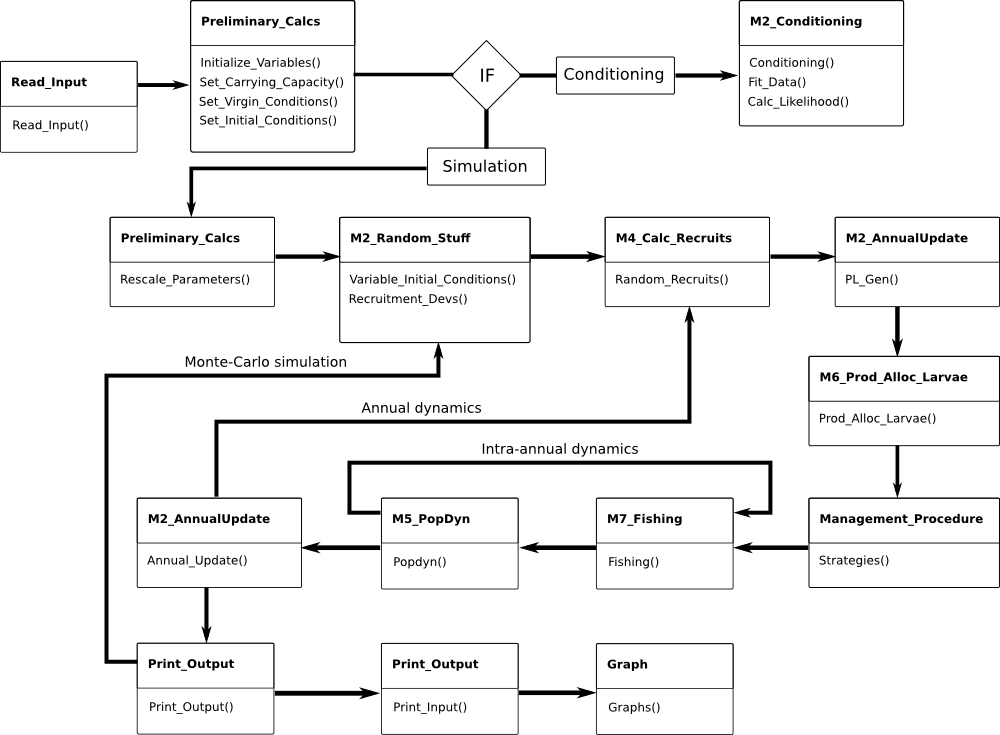
\includegraphics[width=\textwidth]{DiagramaMetapesca.png}
		\caption{Flujo de Ejecución del módulo principal de Metapesca.}
		\label{fig:FlujoEjecucion}
		\end{center}
		\end{figure}

		En primer lugar, se leen todas las variables de entrada llamando al módulo \emph{Read\_Input} y se almacenan en variables globales definidas en el módulo \emph{M1\_VarDef}. 
		Seguidamente se llama al módulo \emph{Preliminary\_Calcs} y se ejecutan los procedimientos que inicializan variables (\emph{initializeVariables()}), los que determinan las condiciones bajo las que estaría un población virgen no explotada (\emph{setVirginConditions()}) y las condiciones iniciales de las que va a partir el modelo (\emph{setInitialConditions()}). 
		Una vez realizados estos cálculos, hay una bifurcación en el modelo en función de si se quieren estimar los parámetros del modelo o realizar simulaciones. 
		Para ajustar el modelo a datos históricos se ejecuta \emph{M2\_Conditioning}. 
		Si se quieren llevar a cabo simulaciones se reescalan los parámetros (en función del intervalo de tiempo intra-anual elegido), se añade un componente aleatorio a las condiciones iniciales y se calculan las desviaciones del reclutamiento (módulo \emph{M2\_Random\_Stuff}). Allí se da inicio al ciclo anual. Éste comienza con el reclutamiento y la producción de larvas (módulo \emph{M6\_Prod\_Alloc\_Larvae}), que se distribuyen entre áreas de acuerdo a una matriz de conectividad. Luego sigue con el proceso de pesca (módulo \emph{M7\_Fishing}), el crecimiento y la mortalidad (módulo \emph{M5\_Popdyn}). Si la dinámica ocurre a una escala temporal menor que la anual (por ejemplo mensual), los módulos \emph{M7\_Fishing} y \emph{M5\_Popdyn} se repiten en los ciclos de dinámica intra-anual. 
		\par La pesca está regulada de acuerdo a reglas de manejo definidas en el procedimiento \emph{Strategies()} del módulo \emph{Management\_Procedure}.   
		Al final de cada ciclo anual, en la rutina \emph{AnnualUpdate()}, se calculan todos los totales de biomasas y se guardan las variables de abundancia a la edad, abundancia, talla y peso a la edad. 

		Una vez simulados todos los años se generan 'salidas' para todo el periodo de tiempo.
		Para cada una de las simulaciones de Monte Carlo a realizar se repite todo el proceso desde el cálculo de las condiciones iniciales variables y las desviaciones en el reclutamiento. 

		Al finalizar, se grafican los resultados.
		
		\subsection{Preliminary\_Calcs}
			\paragraph{Initialize\_Variables()}
				Subrutina. Inicializa las variables que son combinaciones de otras variables obtenidas en el Input. 
			\paragraph{Set\_Carrying\_Capacity()}
				Cálcula la composición poblacional en capacidad de carga. 
					\begin{enumerate}
						\item Distribuciones de tamaños: Asume que los individuos de cada clase de edad se distribuyen normalmente con media $\mu$ y desviación típica $\sigma$. Para el grupo 'Plus' se calculan el tamaño medio (ponderando los tamaños medios por edad por el número de individuos) y los porcentajes de cada tamaño (también ponderando por el número de individuos). 
						\item Abundancias y biomasa por edad. Asume que la población sólo pierde individuos por mortalidad natural ($N_{t+1}=N_t e^{-M}$)
						\item Reclutamiento: Calculo de la biomasa por recluta (BR0) para cada área y del reclutamiento vírgen ($R_0$) en base a la capacidad de carga (parámetro de entrada)bajo condiciones  
						\item Biomasa madura (para calcularla necesita la fracción de maduros (FracMat) y llama a \emph{M5\_Popdyn.Maturity()}) y biomasa vulnerable a la pesca. 
						\item Calcula la productividad (por unidad de biomasa desovante) de la población en condiciones vírgenes. 
						\item Imprimir condiciones de capacidad de carga en hoja de cálculo \emph{Carrying\_Capacity}. 
					\end{enumerate}
			\paragraph{Set\_Virgin\_Conditions()}
			Calcula las condiciones de equilibrio de la población virgen, que no son iguales a las de capacidad de carga si el aporte de larvas a alguna de las áreas está limitado. 
			Para ello realiza una simulación de 200 años partiendo de una población en capacidad de carga y escribe los resultados en la hoja \emph{Virgin\_Conditions})
			\paragraph{Set\_Initial\_Conditions()}
			Cuatro alternativas dependiendo del valor de \emph{RunFlags.Initial\_Conditions}: 
				\begin{enumerate}
					\item Población en capacidad de carga.
					\item Población en equilibrio sin explotar.
					\item Población explotada con tasa constante. Realiza una simulación de 200 años partiendo de una población vírgen y toma los valores finales como condiciones iniciales de la simulación. (Escribe las condiciones iniciales en \emph{Initial\_Conditions})
					\item Lee las condiciones iniciales desde archivo/hoja de cálculo (\emph{Initial\_Conditions}).
				\end{enumerate}
			Los tres primeros procedimientos escriben las condiciones iniciales en la hoja de cálculo \emph{Initial\_Conditions()} (el último no porque ya están ahí escritas).
				
			\paragraph{Rescale\_parameters()}
			Cambia la escala de la mortalidad natural, y parámetros de crecimiento anuales en función del número de intervalos temporales que hay dentro de un año (Nt).
		
			
			
		\subsection{M2\_Random\_Stuff}
			\paragraph{variableInitialConditions()}
				A partir de los valores iniciales se generan nuevos valores introduciéndoles un error multiplicativo $ln(\varepsilon) \in N(0,\sigma)$.
				 \par Bajo estas condiciones, el mejor estimador de la media es $e^{\mu+\frac{\sigma^2}{2}}$ y el mejor estimador de la mediana es $e^{\mu}$. La media va a variar en función de $\sigma$ mientras que la mediana es independiente de la varianza de los errores. 
				\par Por lo tanto, a fin de que la media de los reclutamientos simulados sea independiente de la variabilidad asumida, se trabaja con:
				$\varepsilon=e^{\mu-\frac{\sigma^2}{2}}$, 
				donde $\mu= Z\in N(0,1) \cdot \sigma$
				\par El mejor estimador de varianza en una log-normal es $\hat{S}^2=(e^{\sigma^2}-1)e^{2\mu+\sigma^2}$. Sabiendo que el coeficiente de variación $C_V=\frac{\hat{S}}{\bar{\varepsilon}}$, se cumple que en los casos en los que la varianza es pequeña (del orden de 0.x), $C_V \approx \sigma$. Por lo que en este caso se trabaja con los coeficientes de variación.
				\par Se calcula $N_t$ multiplicándolo por $\varepsilon$ y después se recalculan los Btotal, Bmature, Bvulnerable. Se reinician las variables temporales necesarias para comenzar las simulaciones (NTmp, BvulTmp, etc.). Se vuelve a hacer la survey parcial si procede llamando al procedimiento DoSurvey() y se le asignan al Atlas[ ] los valores de la evaluación. 
			
			\paragraph{recruitmentDevs()}
				Calcula las variaciones en el reclutamiento introduciéndoles correlación temporal según $\varepsilon_{t+1}= \rho \varepsilon_t + Y_t$ donde $Y \sim N(0, \sigma_{\varepsilon} \sqrt{1-\rho^2})$. 
				Asi $Y_t= \sigma_{\varepsilon} \sqrt{1-\rho^2} Z$.
				NOTA:Habría que hacer también correlaciones espaciales. Mirar como hacerlo con algebra de matrices.
				
			
		\subsection{M4\_Calc\_Recruits}
			Calcula el número de reclutas. Este módulo tiene tres procedimientos:\begin{inparaenum}[(i)] \item \emph{Deterministic\_Recruits()} se utiliza durante el cálculo de las condiciones vírgenes y de las condiciones iniciales bajo tasa de explotación constante, \item \emph{Random\_Recruits()} se utiliza durante las simulaciones de Monte-Carlo, \item \emph{Tunned\_Recruits()} toma índices de reclutamiento de un archivo (se utiliza en el conditioning) \end{inparaenum}.
			Dentro de estos tres procedimientos hay dos opciones: 
					\begin{enumerate}
						\item Reclutamiento constante. 
						\item Compensacion lineal.
					\end{enumerate}
			Estas opciones van ser muy similares en los dos primeros procedimientos, diferenciándose sólo en si se les añade o no un error. Calculan el número de reclutas, a partir del los \emph{settlers} (número de individuos que se asientan), y los van a pasar al número de invididuos de la primera clase de edad. Con esto se recalculan las biomasas totales (madura, vulnerable, total).
			\paragraph{Random\_Recruits()} 
				Dos opciones: 
					\begin{enumerate}
						\item Reclutamiento constante: $N_{t,i,edadinicial}= R_0 \cdot e^{Rdev-0.5 RecCV^2}$.
						\item Compensación lineal: $N_{t,i,edadinicial}=Settlers \cdot e^{Rdev-0.5 RecCV^2} $. Y está limitado a ser menor o igual que el menor de la $\frac{K - Btotal}{w_0}$ (condicionado a ser igual o mayor que cero) y el reclutamiento máximo que puede albergar el área($RMax$).
					\end{enumerate}
				
			
		\subsection{M2\_Annual\_Update.pLgen()}
			\paragraph{pLgen()}
				Genera los pL[], es decir el porcentaje de individuos de cada talla que hay en la población
		\subsection{M6\_Prod\_Alloc\_Larvae}
			\paragraph{Prod\_Alloc\_Larvae()}
				Calcula las larvas para cada año ($Bmature[year, area]* ProdXB$) y las reparte de acuerdo a la matriz de conectividad. Estas corresponden al número de individuos que llegan a cada área para asentarse en el año $t+Stage$, es decir después de que pase el suficiente tiempo como para que se recluten.  
				NOTA: Los settlers desde \emph{t=Año de Inicio} hasta \emph{t=(Año de inicio + Edad de reclutamiento-1)} ya se han calculado dependiendo de las condiciones iniciales de las que se parten. 
		\subsection{Management\_Procedures}
			\paragraph{Strategies()}
			Este procedimiento es el encargado de realizar las surveys (globales o parciales) si procede, de pasar las áreas a pescar a estado 'Abierto' (ClosedArea = False), y de generar un vector temporal(\emph{ClosedAreaTemp}) que especifica si dichas áreas están cerradas o abiertas y que le sirve de input al método \emph{Fishing()}. Además, ajusta la HarvestRate en caso necesario (que implicaciones en el manejo conllevaría esto, i.e., el hecho de que tengas que ajustar la harvest rate para no pasarte de los límites, ¿qué implicaría en el caso real?).
				Tres estrategias distintas:
					\begin{enumerate}
						\item Rotaciones. 
							\begin{enumerate}
								\item Se cierran todas las áreas a la pesca. 
								\item Si hay cuotas de captura.
									\begin{enumerate}
										\item Si hay feedback se realizan las evaluaciones de las áreas o, en el caso de que sean evaluaciones parciales, se calcula la cuota multiplicando la abundancia estimada por la harvest rate.
										\item Se van abriendo las áreas que cumplen la condición de reapertura (si hay, sino por orden).
										\item Se calculan el número de áreas que se van a pescar (Nfishedareas).
										\item Si la captura esperada sobrepasa la cuota se ajusta la HR. 
									\end{enumerate}
								\item Si hay cuotas de esfuerzo: No hace nada porque aún no se ha implementado. 
								\item Si es por tasas de explotación: Se hace abriendo sólo el porcentaje de la supercifie explotable que se correspondería con la harvest rate objetivo. 
								\begin{enumerate}
									\item Se abren las áreas que se van a pescar.
									\item Se cuenta cuantas son (Nfishedareas).
								\end{enumerate}
							\end{enumerate}
						\item Gestión por área
							\begin{enumerate}
								\item Si hay feedback se realizan las evaluaciones de las áreas (llamando a \emph{DoSurvey()}), y:
								\begin{enumerate}
									\item Si hay cuotas de captura: Se calculan las TACs por área (\emph{TAC\_area}).
									\item Si hay cuotas de esfuerzo: Hay que implementar una rutina que te calcule los \emph{TAE\_area[]}.
								\end{enumerate}
							\end{enumerate}
						\item Gestión regional
							\begin{enumerate}
								\item Si hay feedback se realizan las evaluaciones de las áreas (llamando a \emph{DoSurvey()}), y:
								\begin{enumerate}
									\item Si hay cuotas de captura: Se calculan las TACs por región (\emph{TAC\_region[]}).
									\item Si hay cuotas de esfuerzo: Hay que implementar una rutina que te calcule los \emph{TAE\_region[]}.
								\end{enumerate}
								\item Se calculan los EffortPulse (para el caso de TAEs y el resto). 
							\end{enumerate}
					\end{enumerate}
			Para todos los casos se calcula al final de la rutina los \emph{ClosedAreaTmp} para todas las áreas, que se le pasan al \emph{Fishing()}.
				
		\subsection{M7\_Fishing}
			\paragraph{Fishing()}
				Realiza las extracciones para cada pulso de pesca, calculando las capturas anuales por área. 
				Tres casos:
				\begin{enumerate}
					\item Rotaciones. Mira si el área está abierta, ajusta las tasas de explotación si es necesario, si hay survey parcial ajusta los Atlas y después calcula las capturas. 
					\item Por Área. Mira si las áreas están abiertas a la pesca, y si lo están:
						\begin{enumerate}
							\item Si hay cuotas de captura: Calcula la harvest rate, y después las capturas (si la harvest rate es mayor que 0.9 se toma como 0.9 y de ahí se sacan las capturas. 
							\item Si hay cuotas de esfuerzo: Entonces la $HR=1-e^{-Q(Area)*TAE}$ y de ahí se calculan las capturas.
							\item Si es por tasa de explotación: Se calculan las capturas a partir de esa tasa. 
						\end{enumerate}
					\item Por Región
					 \par Si es por harvest rate el programa no permite hacerlo, ya que considera que es análogo al caso de manejo por áreas y que debes utilizar esa opción. Sale un mensaje de aviso indicándote que cambies la opción a manejo por áreas.
					\par Se va a poder realizar la distribución de la pesca entre áreas mediante varias estrategias, determinadas por el valor de \emph{EffortDistributionFlag}:
					\begin{enumerate}
						\item Ideal Free Distribution según el algoritmo 'obsoleto' o mediante la repartición del esfuerso en trozos o cachitos. 
						\begin{enumerate}
							\item Si hay cuotas de captura: IFD hasta que se llegan a las distintas cuotas por región.
							\item Si hay cuotas de esfuerzo: IFD dentro de cada región, para repartir ese esfuerzo entre áreas. 	 
						\end{enumerate}
						\item Ideal Free Distribution basada en el algoritmo de Walters \& Martell (2003). 
						\begin{enumerate}
							\item Si hay cuotas de esfuerzo: Se aplica el algoritmo de Walters para cada región y se reparten los esfuerzos calculados homegéneamente a lo largo de toda la temporada de pesca. NOTA: Con esto se podría jugar mirando que estrategias de repartición del esfuerzo a lo largo del año serían mejores (e.g. pescarlo todo al principio o esperar al final).
							\item Si hay cuotas de captura: En ello. Está implementado para el caso en el que haya una única región. 
						\end{enumerate}
						\item Gravitacional (No implementada)
					\end{enumerate}

				\end{enumerate}
		\subsection{M5\_Popdyn}
			Este módulo se encarga de hacer crecer y morir (mortalidad natural) a los individuos. 
		
				\paragraph{PopDyn()} Se determina la g (fracción de reducción) del crecimiento. 
				Si una edad no está reclutada o está parcialmente reclutada, se calcula en dónde se encuentra con respecto a la talla vulnerable (estándarizando y mirando la probabilidad equivalente de una $N(0,1)$. Si empieza a ser vulnerable Flag\_Rec\_Fish pasa a ser 2 y si ya es totalmente vulnerable 3.  
		
				El crecimiento puede se linealmente dependiente o independiente.
				Flag\_Rec\_Fish puede tener tres valores. 1 (por defecto) indica que la edad no ha sido reclutada. 2 que ha sido parcialmente reclutada y 3 que está totalmente reclutada. Según el estado de cada edad, se va a llamar a Norm (no reclutada) o Trunc\_Norm (el resto de casos) para determinar la estructura de tallas de cada edad. 
				
				La clase de edad AgePlus se calcula de forma diferente, haciendo crecer los distintos intervalos de talla y asignando a esos individuos a su clase de talla final correspondiente. Así, se calcula para cada intervalo de talla un Lplus que se corresponde con el tamaño que tendrían los individuos de esa talla después de crecer, y se mira en que intervalo de tallas quedarían.  
				
				Se calculan las FracSel, biomasas y pesos para el intervalo de tiempo siguiente. 
				
				Como la biomasa cambia al crecer los individuos, hay que controlar que no se sobrepase la capacidad de carga del medio, y en el caso que se sobrepase aumentar la mortalidad. Al tratarse de un modelo discreto, si se espera a que se llegue a capacidad de carga para aumentar la mortalidad, se van a generar ciclos de reclutamiento-no reclutamiento (ya que cuando llega a capacidad de carga no hay sitio para más individuos y no habría reclutamiento), para 'suavizar' este proceso y adecuarlo más al caso diferencial, lo que se hace es asumir que hay una capacidad de carga de adultos de la forma:
				\begin{equation}
					K_{adultos}= K - R_0 Peso_{inicial}
				\end{equation}
				  
				 Donde $K$ es la capacidad de carga del medio, $R_0$ es el reclutamiento en condiciones vírgenes (donde se asume que la población está en equilibrio, y el reclutamiento es el mínimo necesario para sustentar a la población y que este equilibrio se mantenga), y $Peso_{inicial}$ es el peso medio por recluta. 
				 
				 Partiendo de esta $K_{adultos}$ se calcula la mortalidad extra que hay que aplicarle a la población en el caso de que esta capacidad de carga se vea sobrepasada, de tal forma que:
				\begin{equation}
					XtraM= \frac{K_{adultos}}{B_{total}} 
				\end{equation}
				 XtraM sería la reducción en la supervivencia de los individuos si la $K_{adultos}$ se sobrepasa. Y esta se multiplica por la BtotTmp, BvulTmp y NTmp.
				
		\subsection{M2\_AnnualUpdate}
			\paragraph{AnnualUpdate()} Actualiza las variables temporales y las mueve de un año al siguiente. 
			
		\subsection{Print\_Output}
			\paragraph{printOutput()} Imprime los resultados de la simulación en las hojas de cálculo correspondientes.
			
		\subsection{Graphs}
			\paragraph{Graphs()} Se encarga de crear los gráficos de salida. En concreto:
				\begin{enumerate}
					\item Catch vs. Time
					\item Effort vs. Time
					\item Vulnerable biomass vs. Time
					\item Spawning biomass vs. Time
					\item Larvae vs. Time
					\item Density vs. Time
					\item Recruits vs. Time
					\item Total biomass vs. Time
					\item Harvest Rate vs. Time
					\item Depletion en la biomasa vulnerable vs. Time
					\item Depletion en la biomasa de maduros vs. Time
				\end{enumerate}
		
		
		

	\section{Library Functions}
	
	\paragraph{Norm(Area, Age)} Calcula las probabilidades que tendría cada clase de talla según una normal $N(\mu, \sigma)$. Como las clases de talla son valores discretos se divide cada probabilidad entre el sumatorio de todas ellas, para que la distribucion de las probabilidades vaya de $0$ a $1$.
	\paragraph{Cumd\_Norm(x)} Calcula la probabilidad acumulada desde $-\infty$ a $x$ según una $N(0,1)$.
	\paragraph{Trunc\_Norm(Area, age)} Calcula las probabilidades que tendría cada clase de talla según una normal $N(\mu, \sigma)$, truncando la función en los puntos en los que hay discontinuidades debido a los pulsos de pesca.

		

